% !TEX root = ../main.tex
\documentclass[../main.tex]{subfiles}
\begin{document}
\section{Компьютерная модель распространения звука в легких}
\subsection{Математическая модель}
В рамках данной магистерской работы была разработана и протестирована компьютерная модель распространения звука в легких.

Модель строится на следующих предположениях
\begin{enumerate}
    \item среда ведет себя как жидкость (80\% тела является жидкостью)
    \item среда неподвижна
    \item полное отражение на границах тела
\end{enumerate}

В качестве математической модели распространения звука было взято волновое уравнение для неоднородной среды.

\begin{figure}[H]
\centering
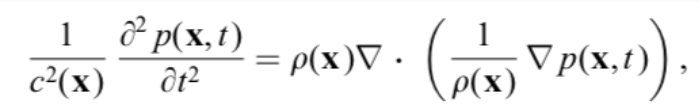
\includegraphics[width=\textwidth]{images/waveeq}
\caption{волновое уравнение для неоднородной среды}
\end{figure}

\begin{itemize}
    \item $p(x, t)$ - давление воздуха (pressure)
    \item $\rho(x)$ - плотность ткани / мышц
    \item $c(x)$ - скорость звука
    \item $x = [x, y, z]$ - точка пространства
\end{itemize}

Начальные условия для данной модели:

Предполагаем что в нулевой момент времени давление равно нулю во всех точках. В качестве альтернативы можно использовать атмосферное давление. Для всех $x$:

$$p(x, t=0) = 0$$

производные давления для всех координат по времени в момент времени $t=0$ также равны нулю:
$$\frac{\partial p(x, t)}{\partial t} \rvert t=0 = 0$$

Также присутсвует условие затухания звука: (включая затухания на границах тела).

В качестве источника звука в течении первых нескольких секунд генерируется синусоидальная волна для давления:

$$p(a, b, c, t) = sin(2 \pi f t)$$

где $x = (a, b, c)$ - положение источника звука. $f$ - частота в Герцах.

Приведенное выше волновое уравнение для неоднородной среды решалось численным приближением при помощи метода конечных разностей. Производные заменялись на разность, давление в точке в последующий момент времени считалось как сумма давлений окружающих ее точек (с коэффициентами). В итоге формула для давления в точке $i, j, k$ в момент времени $m + 1$ выглядит следующим образом:

$$\kappa_{ijk} = \frac{l}{h}c_{ijk}$$
$$l = \Delta t$$
$$h = \Delta x = \Delta y = \Delta z$$

\begin{figure}[H]
\centering
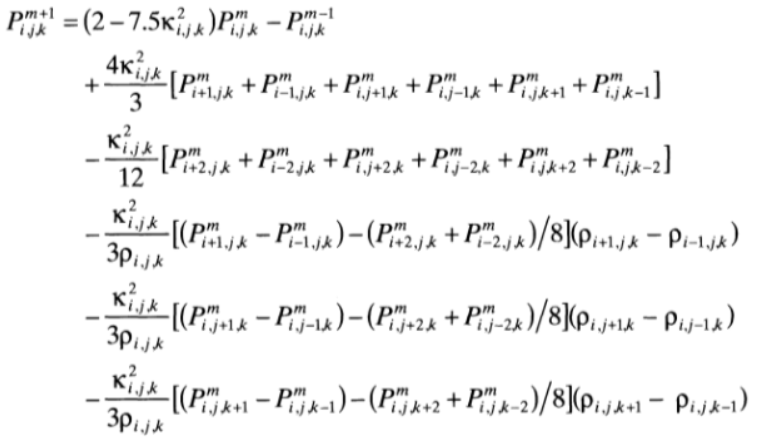
\includegraphics[width=\textwidth]{images/numeric}
\caption{численное приближ. решение волнового уравнения для неоднородной среды}
\end{figure}

\subsection{Human Visible Project Dataset}
Особенностью данной модели является то, что она основана на реальных данных. В модели использовался датасет снимков компьютерной томографии Human Visible Project Dataset. Данный датасет представляет собой 1,871 изображений. Каждое изображение это снимок компьютерной томографии. Снимки делались с инервалом 1 милиметр друг от друга вдоль вертикали туловища.

\begin{figure}[H]
\centering
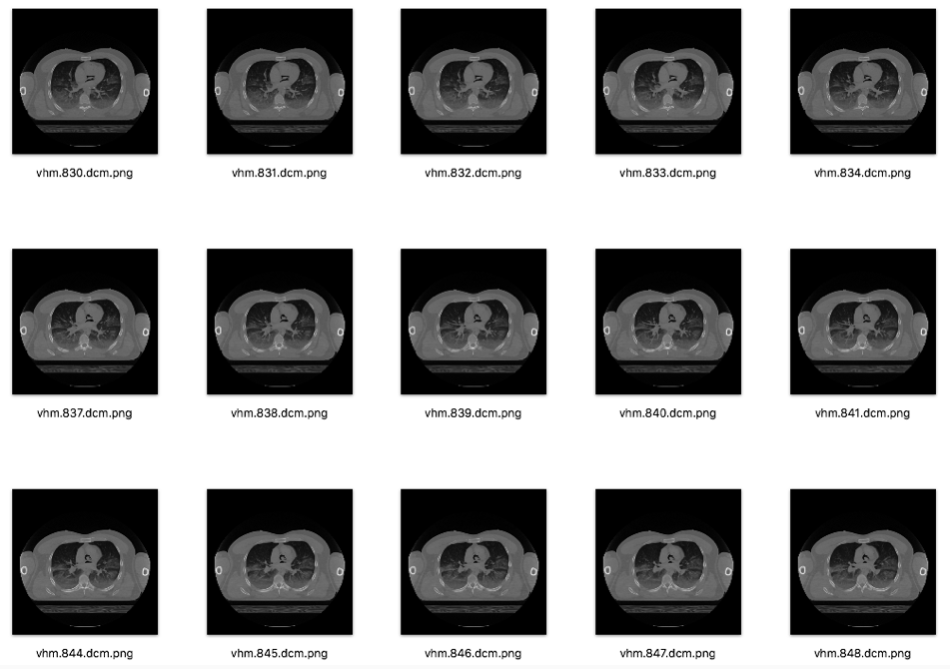
\includegraphics[width=\textwidth]{images/hvp}
\caption{датасет снимков компьютерной томографии Human Visible Project}
\end{figure}
Из данного датасета были выбраны только те снимки, которые отвечают за область легких.

Компьютерные снимки содержат информацию о яркости а для модели нужна плотность. Чтобы перевести значения яркости снимков в плотность использовалась следующая таблица:

\begin{center}
\begin{tabular}{ |r|r| } 
 \hline
 Яркость CT & Плотность \\
 0     & 0.000 \\
 20    & 0.001 \\
 254   & 0.292 \\
 444   & 0.438 \\
 944   & 0.895 \\
 957   & 0.945 \\
 986   & 0.980 \\
 1024  & 1.000 \\
 1139  & 1.116 \\
 1211  & 1.142 \\
 1504  & 1.285 \\
 1884  & 1.473 \\
 2307  & 1.707 \\
 4000  & 2.213 \\
 15160 & 4.510 \\
 43410 & 7.850 \\
 \hline
\end{tabular}
\end{center}

\subsection{Компьютерная программа на основе математической модели}
Компьютерная программа представляет собой кросплатформенное Desktop - приложение, написанное на языке python с использованием графического фреймворка PyQt. Для работы с многомерными массивами использовалась библиотека Numpy.

Компьютерная модель была реализована как для двухмерного так и для трехмерного случая. В двухмерном случае берется 1 снимок из датасета. В трехмерном случае все снимки легких были "склеены" в один трехмерный массив, который был сохранен в бинарный файл с расширением \texttt{.npy}. Это стандартный для numpy способ сериализации данных. Данный формат очень быстро загружается в память и превращается в массив \texttt{numpy.ndarray}.

С точки зрения программирования модель представляет собой 2 класса: один отвечает за графический интерфейс пользователя, другой - собственно за модель.

Класс модели хранит состояния следующих переменных в текущий момент времени а также 2 шага назад:

\begin{itemize}
    \item состояние плотности для всех точек
    \item состояние давления для всех точек
    \item состояние скорости звука для всех точек
\end{itemize}

Также в данном классе можно задать частоту, местоположение и длительность начального звука который будет распространяться по легким. Инициализация переменных начальными значениями или параметрами по умолчанию происходит в методе \texttt{\_\_init\_\_}. Метод \texttt{step} расчитывает состояние системы на один временной шаг вперед. Метод \texttt{update\_P} обновляет значение плотности на основе двух предыдущих значений плотности.

Графический интерфейс представляет собой окно c несколькоми графиками и элементами управления. Основные три графика, находящиеся по центру окна - это срезы легких в трех проекциях: X, Y, Z. На эти срезы накладывается график отвечающий за плотность звука. 

Над графиками располагаются 3 слайдера, позволяющие перемещать срезы в проекциях. Слайдеры обозначены цветами, соответсвующие цвета присутсвуют на срезах и показывают их местоположение.

Ниже присутсвуют 3 графика, позволяющие посмотреть давление в трех произвольных точках за последние 100 временных шагов. Присутсвует кнопка, позволяющая сделать переход модели на 1 временной шаг вперед. Также есть возможность задать количество шагов и запустить модель.

Присутсвуют элементы управления основными параметрами модели: частотой генерируемой звуковой волны, положение источника звука, временной шаг в секундах. Есть кнопка которая сбрасывает параметры на значения по умолчанию.

\begin{figure}[H]
\centering
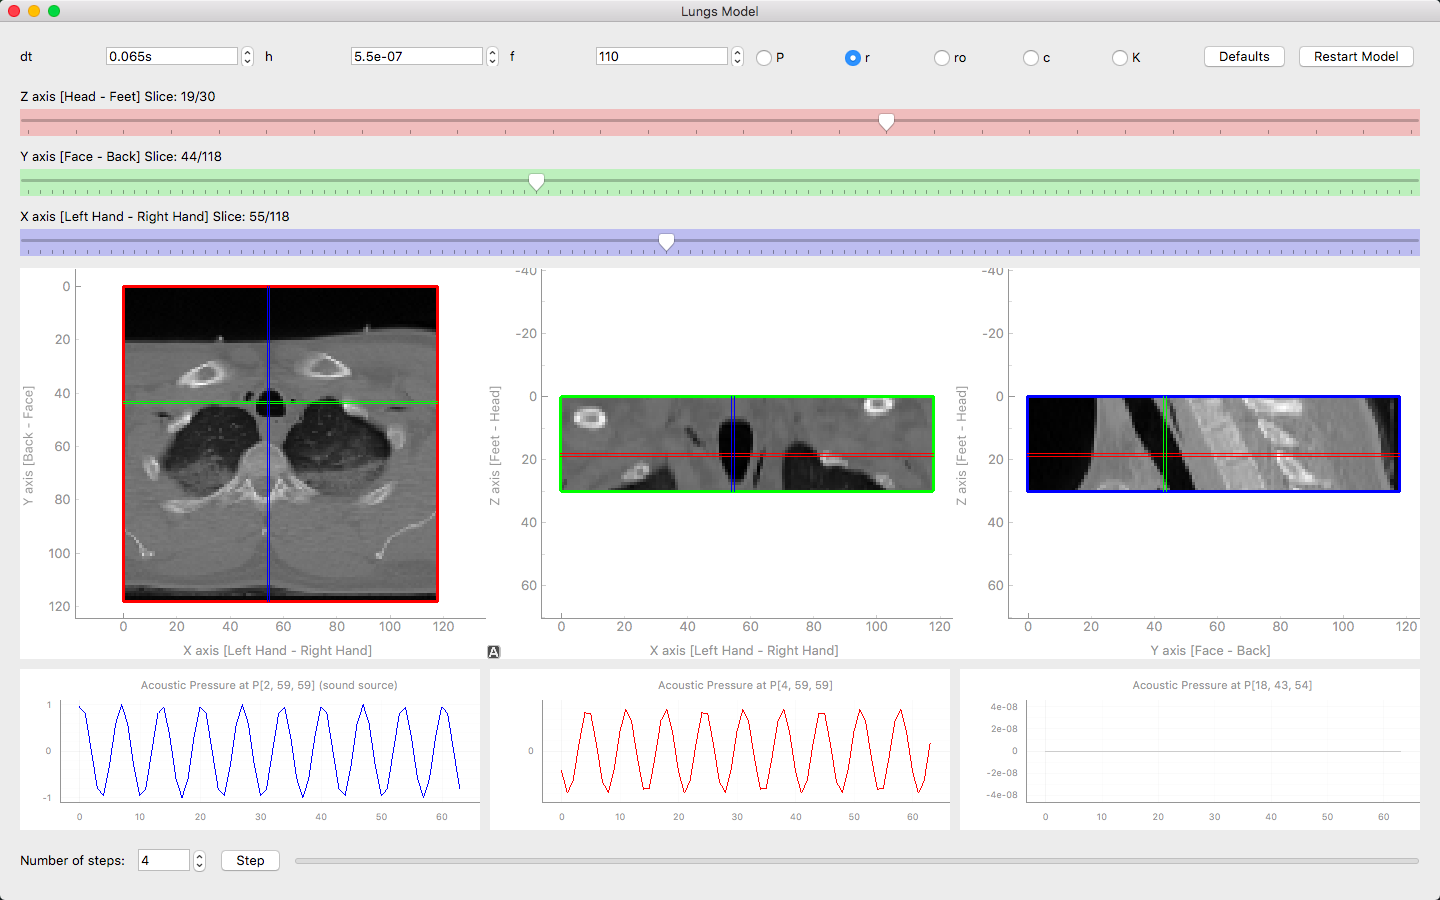
\includegraphics[width=\textwidth]{images/3d-lungs}
\caption{Трехмерный вариант компьютерной модели распространения звука в легких}
\end{figure}


Также был реализован двухмерный вариант модели. Двухмерный вариант позволяет более наглядно наблюдать распространение звука.


\begin{figure}[H]
\centering
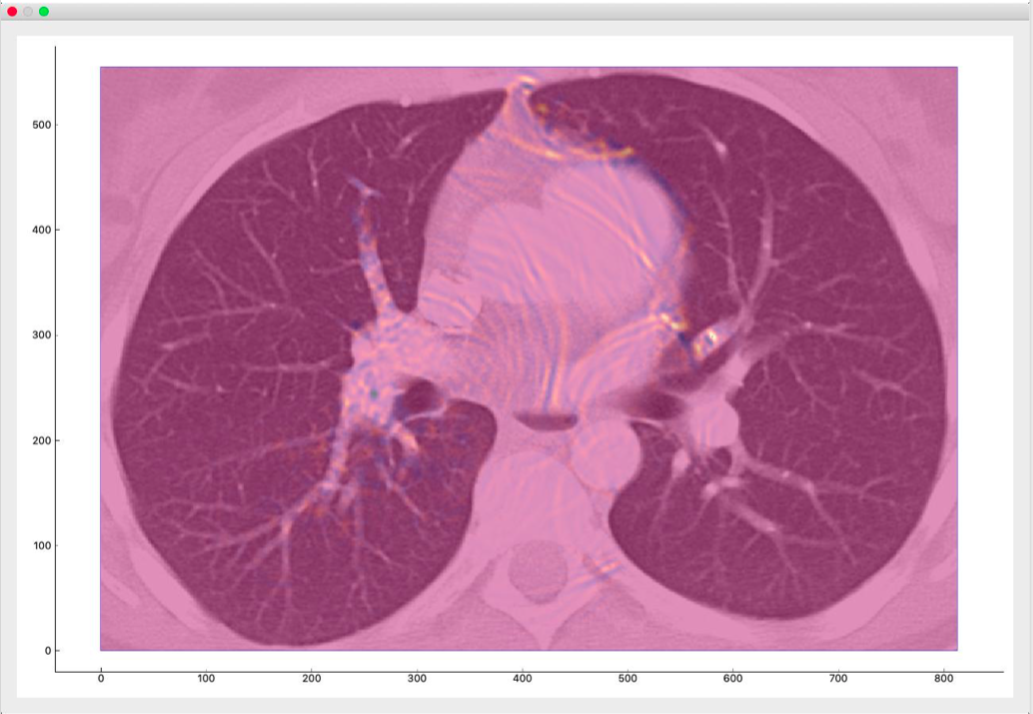
\includegraphics[width=\textwidth]{images/2d-lungs}
\caption{Двухмерный вариант компьютерной модели распространения звука в легких}
\end{figure}

Более подробно результат работы модели можно посмотреть на видео \cite{lungs-2d-youtube}

Полный код компьютерной модели легких можно посмотреть в приложениях 1 и 2:
\begin{itemize}
    \item \hyperref[appendix1]{Приложение 1 -  класс LungsModel}
    % \item \hyperref[appendix1]{Приложение 1 -  класс \verb|LungsModel|}
    \item \hyperref[appendix2]{Приложение 1 -  класс AppGUI}
    % \item \hyperref[appendix2]{Приложение 1 -  класс \verb|AppGUI|}
\end{itemize}
 

\newpage
\end{document}
